% !TEX root = ../main.tex

% = = = = = = = = = = = = = = = = = = = = = = = = = = = = = = = = = = = = = = = = = = = = = = %

\section{Introduction}

Bitcoin~\cite{nakamoto2008bitcoin} emerged almost a decade ago as an open source project, which mushroomed into a cryptocurrency sector collectively capitalized at over \$500 billion USD\footnote{Coinmarketcap - Global Charts - Accessed: 2017-12-14 \url{https://coinmarketcap.com/}}. Every day, people new to the concept of cryptocurrencies look for a quick and simple way to acquire some crypto-wealth. In the early days of Bitcoin, users on their personal computers could effortlessly acquire the currency through mining---a process Bitcoin uses to incentivize nodes to verify transactions as they are recoded in the blockchain. However, a second wave of mining technology saw users augmenting the CPU power of their computers with GPUs. Other groups of people deployed snippets of JavaScript code on websites that recruited their visitor's CPU power, often unknowingly, to mine for them as part of a bigger mining network (\ie a mining pool). However, both approaches quickly became infeasible as the computing power required to mine bitcoins grew exponentially to over 12 petahashes\footnote{Bitcoin hash rate - Accessed: 2017-11-20 \url{https://blockchain.info/charts/hash-rate}}. This was due to the emergence of application-specific integrated circuits (ASICs) and collective mining pools, which continue the third wave of mining to this day~\cite{narayanan2016}. 

\begin{figure}[t]
\centering
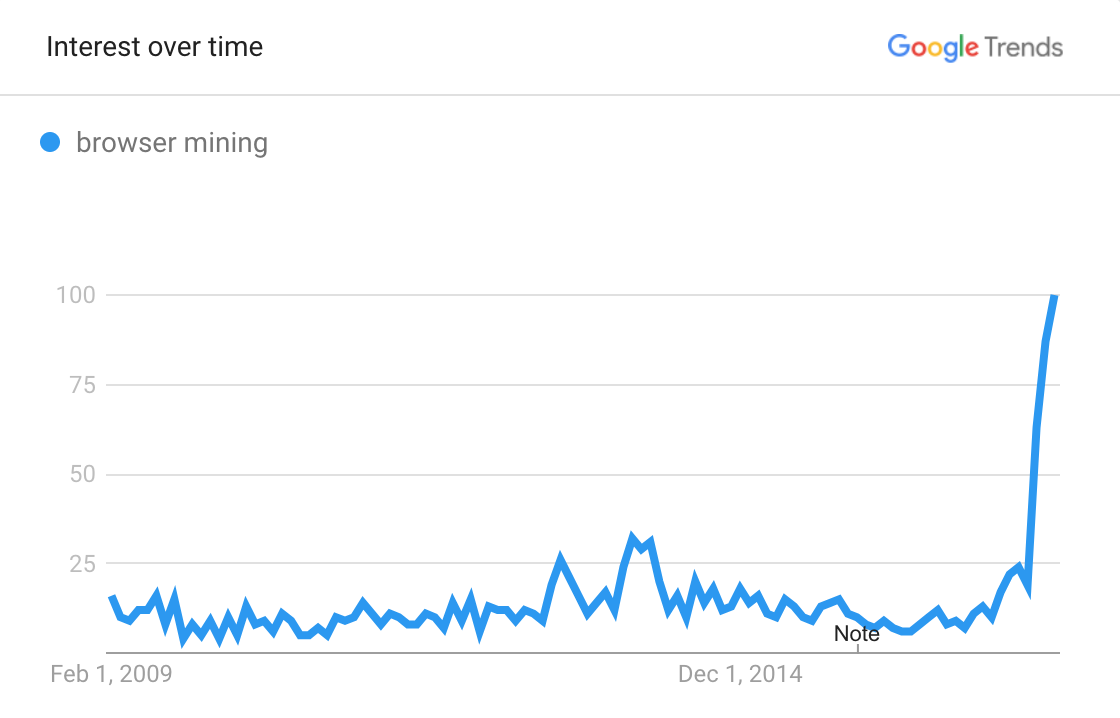
\includegraphics[width=0.9\linewidth]{figures/browser_mining.png}
\caption{Search interest for ``browser mining'' over time. Search interest seems to have piqued during price surges, which culminated with Bitcoin crossing \$1000 USD for the first time in December 2013. Soon after Bitcoin's first major crash searches consistently waned until a recent large spike, which is more than 4 times the lifetime average. The waning period before the recent surge could be attributed to the advent of ASIC usage for Bitcoin mining, and the surge is likely due to the revival of browser mining for non-Bitcoin currencies that have gained a sizeable market capitalization.\label{fig:interest}}
\end{figure}

As the years passed and a few key cryptocurrencies emerged as the market leaders, the concept of browser mining largely became forgotten. Today, the most common way for the average person to acquire cryptocurrencies is to purchase them. It came as a surprise to many when stories began to circulate on popular media outlets this year about websites mining cryptocurrencies through browsers again. Figure~\ref{fig:interest} shows how the searches for ``browser mining'' have changed since Bitcoin was launched. Websites like TIMELINE.org ~\cite{piratesbayhive} experimented with browser mining as a way to add a new revenue stream, while others like Showtime.com ~\cite{showtimehive} claimed they had the code injected after they were discovered. 

This paper tells the story behind the rejuvenation of browser-based mining. It is centred on \textit{cryptojacking} (also known as \textit{coinjacking} and \textit{drive-by mining}), a term coined to refer to the invisible use of a vulnerable user's computational resources to mine cyptocurrencies. Technically in-browser mining is a subset of cryptojacking, although most uses of the term apply to browser-based mining. In this case, mining happens within the client browser when the user visits the website. We have also seen the term cryptojacking applied to malware that mines cryptocurrencies, or in the situation where malware renders a machine as an unwitting participant in a botnet, and the botnet is rented for the purposes of mining crypcurrencies (\cf~\cite{huang2014botcoin}). The resource consumption of in-browser cryptojacking can noticeably degrade a computer's performance.

% = = = = = = = = = = = = = = = = = = = = = = = = = = = = = = = = = = = = = = = = = = = = = = %
%
%
%
%
%
%
% = = = = = = = = = = = = = = = = = = = = = = = = = = = = = = = = = = = = = = = = = = = = = = %

\section{Preliminaries and Related Work}

\subsection{Browser-based Mining}

\subsubsection{Early days}
The idea of in-browser mining started in the early days of Bitcoin. Bitcoin Plus\footnote{Bitcoin For the Uninitiated: Now, A Browser-Based Mining Client  May 19th, 2011 \url{https://www.themarysue.com/browser-based-bitcoin-mining/}} is one example of a discussion on replacing ads with Bitcoin browser miners\footnote{BitCoin browser mining as a replacement for ads \url{https://www.reddit.com/r/Bitcoin/comments/ieaew/bitcoin_browser_mining_as_a_replacement_for_ads/}}. It was also argued that browser-based mining provides greater scalability and decentralization as the barrier to entry is lowered to any unmodified computer with an internet connection. Soon after there was a rise in Bitcoin JavaScript miners such as JSMiner (2011)\footnote{A JavaScript Bitcoin miner \url{https://github.com/jwhitehorn/jsMiner}} and MineCrunch (2014)\footnote{MineCrunch, web(JS) miner with integration feature\url{https://cryptocurrencytalk.com/topic/24618-minecrunch-web-js-miner-with-integration-feature/}}. MineCrunch's visibility was increased by campaigns and the active online presence of its developers. Based on the developer claims, MineCrunch was well optimized for Javascript, but still worked 1.5x slower than native applications for CPU mining (\eg CPUMiner\footnote{CPU miner for Litecoin and Bitcoin - \url{https://github.com/pooler/cpuminer}}). Although CPU mining  became uncompetitive with GPU- and ASIC-based mining, it remained a sandbox for botnet admins to experiment with the thousands of CPUs at their disposal. Botnet mining has been studied in the literature~\cite{huang2014botcoin,wyke2012zeroaccess}, as well as cover mining within enterprises and cloud environments~\cite{MiningonSOeDime2017}.

In addition to unprofitability, browser-based mining faced legal challenges. In May 2015, the New Jersey Attorney General`s office reached a settlement with the developers of ``Tidbit``, a browser-based Bitcoin miner. Terms of the settlement included ceasing operations of Tidbit. Then acting Attorney General John J. Hoffman stated ``No website should tap into a person`s computer processing power without clearly notifying the person and giving them the chance to opt out.`` ~\cite{njcourtbitcoinjsminer}.

\subsubsection{From one CPU to ASICS and mining pools}

<<<<<<< HEAD
The first Bitcoin block mined on a GPU happened on July 18th, 2010 by a user named ArtForz\footnote{bitcoinhistory} using private mining code that he wrote himself. It was not until mid 2011 that others started implementing and releasing open source GPU-based mining tools. These tools greatly increased mining efficiency due to the hashing power of a GPU and the massive parallelizing possible with multiple GPUs (also known as mining rigs). The move from software to hardware followed shortly after. First, programmable FPGA chips resulting in custom-built circuits specifically for mining\footnote{Custom FPGA Board for Sale! (August 18, 2011) \url{https://bitcointalk.org/index.php?topic=37904.0}}. Then by mid 2012, companies started selling ASICs designed specifically for Bitcoin mining. After delay of about a year in delivering ASIC products, Bitcoin mining starting transitioning from GPUs to ASICs where it remains today. Consequently, the hashing power of the Bitcoin network increased and the mining difficulty followed. To illustrate the change, consider a desktop PC CPU mining at 10 MH/s: on expectation, it will take 425 years before mining a single block~\cite{huang2014botcoin}. 
=======
The first Bitcoin block mined on a GPU happened on July 18th, 2010 by a user named ArtForz\footnote{bitcoinhistory} using private mining code that he wrote himself. It was not until mid-2011 that others started implementing and releasing open source GPU-based mining tools. These tools greatly increased mining efficiency due to the hashing power of a GPU and the massive parallelizing possible with multiple GPUs (also known as mining rigs). The move from software to hardware followed shortly after. First, programmable FPGA chips resulting in custom-built circuits specifically for mining.\footnote{Custom FPGA Board for Sale! (August 18, 2011) \url{https://bitcointalk.org/index.php?topic=37904.0}} Then by mid-2012, companies started selling ASICs designed specifically for Bitcoin mining. After delay of about a year in delivering ASIC products, Bitcoin mining started transitioning from GPUs to ASICs where it remains today. Consequently, the hashing power of the Bitcoin network increased and the mining difficulty followed. To illustrate the change, consider a desktop PC CPU mining at 10 MH/s: on expectation, it will take 425 years before mining a single block~\cite{huang2014botcoin}. 
>>>>>>> 15faaadc139a456aba9182ccd3bb9efb6f182aed

In parallel to the evolving technology, collective action emerged through the use of mining pools. A mining pool is a collective of individual miners. Participants receive a slice of work for mining the current block on behalf of the pool. If a member of the pool mines the block, the block reward is split amongst the participants of the pool \textit{pro rata} according to their computational effort. As an aside, a very elegant protocol for reporting `near-solutions' to the pool enables participants to prove, without trust, the level of effort they are contributing to the pool at all times. In general, a mining pools cannot amplify earnings, they only change their shape. An income stream from a pool is a steady trickle, while solo-mining results in sporadic dumps of income. The first Bitcoin block found on a mining pool was on December 16, 2010 that was a beta implementation of a pool operated by a user named \textit{slush}.

\subsection{Monero}

Launched in April 2014, Monero~\cite{monero} is a cryptocurrency alternative to Bitcoin. It purportedly offers increased privacy by obfuscating the participants in a transaction, as well as the amounts. This is in contrast to more popular cryptocurrencies like Bitcoin and Ethereum, where a pseudonymous-but-complete transaction graph can be constructed from the public blockchain. Recent research has shown Monero's obfuscation techniques are less effective than originally claimed~\cite{MMLN17}.  Since regulation on exchanging between cryptocurrencies is lighter than exchanging cryptocurrencies for fiat money, and such services are not geographically bound, obtaining Monero for Bitcoin and vice versa is efficient and enables Monero to be used as a short-term medium of exchange for Bitcoin holders. This approach (and Monero's acceptance) is particularly popular on so-called dark web markets; markets that do not ban illicit goods and services.

A second characteristic that distinguishes Monero from Bitcoin is in the mining algorithm it uses. Monero still employs proof-of-work, specifically an algorithm called CryptoNight~\cite{cryptoknight}. However the computational puzzle is designed to be \textit{memory-hard}: it requires the storage of a large set of bytes and then requires frequent reads and writes from this memory. Such puzzles are optimized for CPUs with low-latency memory-on-chip, and not as well suited for circuits like FPGAs and ASICs. CrypoNight requires approximately 2MB per instance, which fits in the L3 cache of modern processors. Over the course of the next few years, these L3 cache sizes should become mainstream and allow more CPUs, and thus users, to vote in Monero's ecosystem. It has also been shown that ASICs cannot handle more than 1MB of internal memory, which is less than the size of memory required to calculate a new block. GPUs are also at a disadvantage since GDDR5 memory, which are used in modern GPUs and considered one of the fastest types of memory, is notably slower than L3 cache~\cite{van2013cryptonote}.  

% = = = = = = = = = = = = = = = = = = = = = = = = = = = = = = = = = = = = = = = = = = = = = = %
%
%
%
%
%
%
% = = = = = = = = = = = = = = = = = = = = = = = = = = = = = = = = = = = = = = = = = = = = = = %

\subsection{Coinhive}

% !TEX root = ../main.tex

\newcommand\ytl[2]{
\parbox[b]{8em}{\hfill{\color{cyan}\bfseries\sffamily #1}~$\cdots$~}\makebox[0pt][c]{$\bullet$}\vrule\quad \parbox[c]{4.5cm}{\vspace{7pt}\color{red!40!black!80}\raggedright\sffamily #2.\\[7pt]}\\[-2pt]}

\begin{table}
\centering
\begin{minipage}[t]{.7\linewidth}
\color{gray}
\rule{\linewidth}{1pt}
\ytl{2013-10-13}{Monero Cryptocurrency appeared}
\ytl{2017-09-14}{Coinhive Miner launched}
\ytl{2017-09-17}{ThePirateBay caught using coinhive}
\ytl{2017-09-21}{Adblockers started to block coinhive scripts}
\ytl{2017-09-24}{Showtime caught running coinhive}
\ytl{2017-09-25}{Coinhive clones started to appear}
\ytl{2017-10-13}{Politifact website compromised to run Coinhive}
\ytl{2017-10-16}{Coinhive launched authedmine - authorized mining}
\ytl{2017-11-23}{LiveHelpNow Hack incident}
 
% Needs to be completed.
\bigskip
\rule{\linewidth}{1pt}%
\end{minipage}%
\caption{Timeline of Monero and in-browser mining\label{tab:timeline}}
\end{table}


Monero built on its early success and continued to gain in popularity over the years, which caught the attention of some developers who decided to revisit the idea of browser mining. See Table~\ref{tab:timeline} for a timeline of events.  One of the earliest efforts appeared in September 2017 and was called Coinhive~\cite{coinhive}. Soon after a competitor named Crypto-Loot\footnote{Crypto-Loot - A web Browser Miner | Traffic Miner | CoinHive Alternative \url{https://crypto-loot.com/}} emerged. Both websites provided APIs\footnote{Application programming interface} to developers for implementing browser mining on their websites that used their visitors' CPU resources to mine Monero. A portion of mined Monero would go back to the API developer, and the rest would be kept by the website. Not long after their early success, several copycats appeared such as Coin-Have and PPoi~\cite{coinhivecopycats} to take part in the reborn practice. It even inspired a new coin specifically designed for browser mining named JSECoin,\footnote{JSEcoin`s Website Cryptocurrency Mining \url{https://jsecoin.com/}} which has yet to find an audience. These developments took place over the course of a few weeks, which signalled the renewed success of browser mining. However, Coinhive's approach as a legitimate group set it apart from its peers and established itself as the leader in the space. They also launched separate services such as proof-of-work CAPTCHAs and short-links, which could be used to prevent spam while mining Monero~\cite{coinhive}.

% = = = = = = = = = = = = = = = = = = = = = = = = = = = = = = = = = = = = = = = = = = = = = = %
%
%
%
%
%
%
% = = = = = = = = = = = = = = = = = = = = = = = = = = = = = = = = = = = = = = = = = = = = = = %
